\chapter{Results by Condition}\label{ch:results}

FUNCTION: This is the main part of the thesis. Each section varies one quantity while all other
quantities stay at the reference levels (ceteris paribus): agreement, dispersion, goods per agent
at a fixed remainder, the remainder at a fixed number of goods per agent, and the number of agents
at a fixed number of goods per agent and remainder. A final section compares round robin with the
balanced random benchmark and with reversing the last round. Each section ends with a
recommendation and closes with the question that the next one answers.

WRITING TEMPLATE per block (order of paragraphs, NOT subsection headings):
(1) main result with status (proven, measured, conjectured) and main figure: x axis the varied
    quantity, y axis the EFX rate, all other quantities at the reference levels; cell values in
    the surrounding text
(2) does it hold in general? one count over all cells
(3) special cases with proofs, a figure only where needed
(4) how badly round robin fails: survival curves of one cell, one line per level, read off in text
(5) relation to literature, incl. whether EFX existence is proven in these cells
(6) recommendation in one sentence, then one sentence leading to the next block's question
Each block is one file; drop a block by removing its input line.


A: Eine Übersichtsabbildung am Anfang von Kapitel 4, vor Block 1: EFX rate über alle Instanzen gegen $m$, Panels $n$, Spearman 0,48, drei Gini-Linien, dazu grau der balancierte Zufall. Sie dient als Orientierung für alle fünf Blöcke: Man sieht schon den Sägezahn (Block 2), das Niveau nach $n$ (Block 4) und den Abstan

\section{Agreement}\label{sec:agreement}
%% FUNCTION: Shows that round robin achieves EFX less often in a world where agents agree more on
%% what is valuable, and compares round robin with the random baseline. Because agreement hurts
%% more with more agents, the next section turns to the number of agents.

 

 In a world with more agreement, Round Robin achieves EFX less often. Figure~\ref{fig:agreement}
shows the EFX rate against the Spearman rank correlation of the world from which the instances
are drawn, for $n=2,\dots,5$ agents with $m=3n$ goods and three levels of dispersion. All other
quantities are fixed, so the figure varies only agreement. For $n=4$ agents, $m=12$ goods and
Gini $0.52$ ($\theta=1$), the EFX rate falls from $0.741$ at Spearman $0$ to $0.515$, $0.293$ and
$0.109$ at Spearman $0.24$, $0.48$ and $0.73$, and reaches $0.000$ under full agreement. For
Gini $0.28$ ($\theta=0.5$), the rate starts higher but falls in the same way, from $0.913$ to
$0.047$. Only for Gini $0.06$ ($\theta=0.1$) does it stay at $1.000$ at every level of agreement.
Each rate rests on $R=20{,}000$ instances, and the curves are paired, since all levels of
agreement use the same random seeds (Chapter~\ref{ch:model}). This result is measured, not
proven.

\begin{figure}
    \centering
    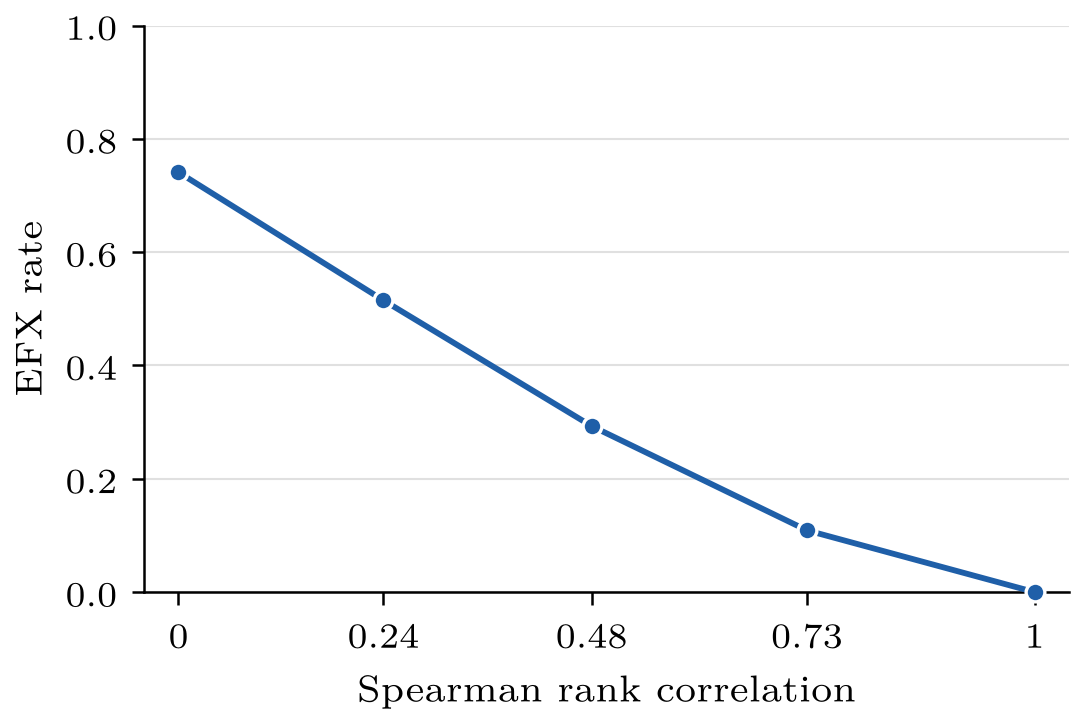
\includegraphics[width=0.6\linewidth]{agreement_rate.png}
    \caption{EFX rate of Round Robin against the Spearman rank correlation of the world from which
instances are drawn, for $n=4$ agents, $m=12$ goods and Gini $0.52$ ($\theta=1$).
Each point rests on $R=20{,}000$ instances.}
    \label{fig:placeholder}
\end{figure}


\section{Dispersion}\label{sec:dispersion}
%% FUNCTION: Shows how the EFX rate of round robin changes with the dispersion of values, all
%% other quantities at the reference levels. Round robin uses only rankings, so its allocation is
%% the same for every level of dispersion; dispersion only changes how this fixed allocation is
%% evaluated. As dispersion vanishes and the number of goods is divisible by the number of agents,
%% the EFX rate tends to one (proven, for every allocation with equal bundle sizes). Since this
%% limit depends on equal bundle sizes, the next section turns to the number of goods per agent.

\section{Bundle Size}\label{sec:bundlesize}
%% FUNCTION: Shows that round robin is guaranteed to be EFX when every agent receives at most two
%% goods and all favourite goods differ, and that this guarantee breaks as soon as one agent
%% receives three goods. Since this break coincides with a change in divisibility, the section
%% leads to the next one.

We define "collision-freeness" as follows: All agents have different favorite goods. The collision rate $1-\#\{distinct favourite goods\}/n$. For $\rho = 1$ it equals to $1-1/n$. Collision-freeness does not occur there.

$\textit{Lemma}$: 

If the instance is collision-free, only Agent $i$ can envy Agent $j$, when $|A_j|>= 3$

Proof: Withtout collision, any agents receives their favourite good in the first round. When $A_j$ only has two goods, after eleminating one good the bundle only has one good left. And that good is not more valuable than his own favourite good. $m=< 2n$ ensures $|A_j| =< 2$

Implication: If the Instance is Collision free and $m=< 2n \Rightarrow RR-Allocation is EFX$

We checked this for every cell. 336 cells with $m=<2n$ and $\rho < 1$, all six $\theta$, 1.388.388 collision free instances, 0 exceptions.

The guarantee does not need an assumption about the distribution.

bitte die tabelle hierhin anteil collsionfree instances.

This condition gets rare quickly. From a ration of 0,749 for ( n =2, rho= 0) to 0,010 for (n=5, rho = 0,75) which only are 193 of 20000 instances.


\begin{figure}
    \centering
    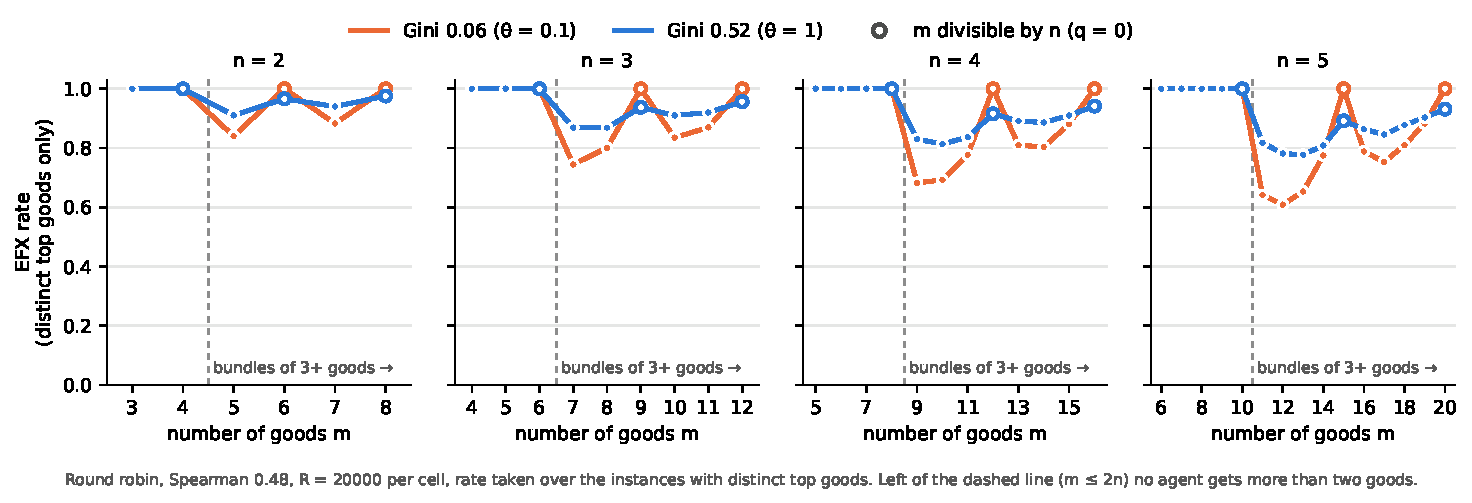
\includegraphics[width=1\linewidth]{block1_fig_break.pdf}
    \caption{Enter Caption}
    \label{fig:placeholder}
\end{figure}

For $n=4$, for $m=<8$ goods, meaning bundle size r=<2 we have a continous EFX Allocation through RR. At 9 goods, we conceive a efx bump to 0,830 (with gini 0,52) and 0,682 (at gini 0,06)
The EFX-quote under kollision free instances show a reocurring pattern that with the divisability of revover.

If we consider all instances however, those trends do not really show in the total graphic.

A bundle with two goods means for the EF1 EFX connection, lead $>=$ gap or "my bundle" $>=$ his best good. and thats secured by the own fav good. 
With three goods now its "my goods vs his two best goods" and the own fav good cannot secure both of them.
Thus, the only endangered pairs are "two vs three goods", for r=2 that are $(n-q) \cdot q$ pairs. 

With smaller $\theta$ is the EFX drop bigger, becaus the structurall lead of the pairs goes to null. 

We assume that the recovery after the drop bc of the growing lead.

Limitations, the depth of the drop also growths with $\rho$ ($n=5$: 0,942 bei $\rho=0$, 0,602 bei $\rho=0{,}75$). The graphic shows the case for $\rho = 0,75$

Another limitation is the assumption about the group we consider itself. in the real world, it rather unusual that everyone has their own favoutie good. It is rather decriptive and based on the quantitave model.

We also have to consider that the gap at 2n+1 can have two infuences.first that for the first time we have a bundle size of 3 but also the rest and divisability goes from 0 to 1. The drop could be the reslut of both changes, however you can split the two effects. becaus for smaller m<=2 there are also q>0  and the efx quote is still 1. The q alone does not break the EFX quote. But this only counts if we only consider the instances where there is collision freeness, considers for all instances this statement does not apply. 

Additionally our Lemma in independet from our distribution bc it only considers the values. If another valuation model creates values where each agents has a own favouite good, this Lemma also applies.

Our emperical foundings also allign with the scientific research, stating that Round Robin has dificouklties of finding ERX with q > 0 with cnstant proability. For an asymptotic case of our collision mechansims \cite{manurangsi2021}.

Also the EFX existance for m=<2n is proved. Moreover \cite{amanatidis2020multiple} prove that there exist and EFX alloctatin until m=<n+3






If every agent receives at most two goods and all favourite goods differ, use Round Robin: EFX is guaranteed, and both conditions can be checked in advance.“ Dazu: Die Bedingung wird mit mehr Personen und mehr Einigkeit schnell selten, und darüber hinaus bricht die Garantie.

How already consideres broadly. A central question is now how the drop behaves with other q's. 
\section{Divisibility}\label{sec:divisibility}
%% FUNCTION: Shows that whether the number of goods is divisible by the number of agents decides
%% the outcome when values are similar. With identical valuations and no divisibility round robin
%% never achieves EFX. The explanation is a structural part of the lead that exists only when all
%% bundles have equal size. The effect fades when values become very unequal, which raises the
%% question of what matters then.


\section{Number of Agents}\label{sec:agents}
%% FUNCTION: Shows that with the same number of goods per agent, EFX becomes rarer as more agents
%% take part, and separates the contribution of colliding favourite goods from the growing number
%% of agent pairs. Since the risk lies with the agents who pick last, the section asks whether a
%% different picking order helps.


\section{Round Robin, Random Allocation and Reversing the Last Round}\label{sec:random}
%% FUNCTION: Compares round robin with the balanced random benchmark that models allocating
%% somehow. With little or moderate agreement, round robin is far ahead. With full agreement and
%% a number of goods not divisible by the number of agents, round robin fails EFX with certainty
%% (proven), while random allocation fails only almost always. Reversing the last round, which is
%% just as easy to carry out by hand, removes exactly the pairs at which round robin fails there
%% (known results) and helps substantially when agents receive few goods or values are similar
%% (measured, exploratory).

% Dropped 10.11.: \section{Picking Order}\label{sec:sequences}
%% FUNCTION: Compares round robin with three simple variants of the picking order that are just as
%% easy to run by hand. It shows where they improve the EFX rate and why the largest gains come
%% from who receives the extra goods. This section is exploratory.


